\chapter{Marco Teórico}

\section{Arquitectura del sistema}

En la figura~\qref{fig:dude-arq} se pueden apreciar los componentes del sistema y cómo interaccionan entre ellos. Además se puede observar los protocolos que utilizan para estas interacciones, a continuación se presentarán los conceptos básicos del sistema.

\begin{figure}[h!]
  \centering
  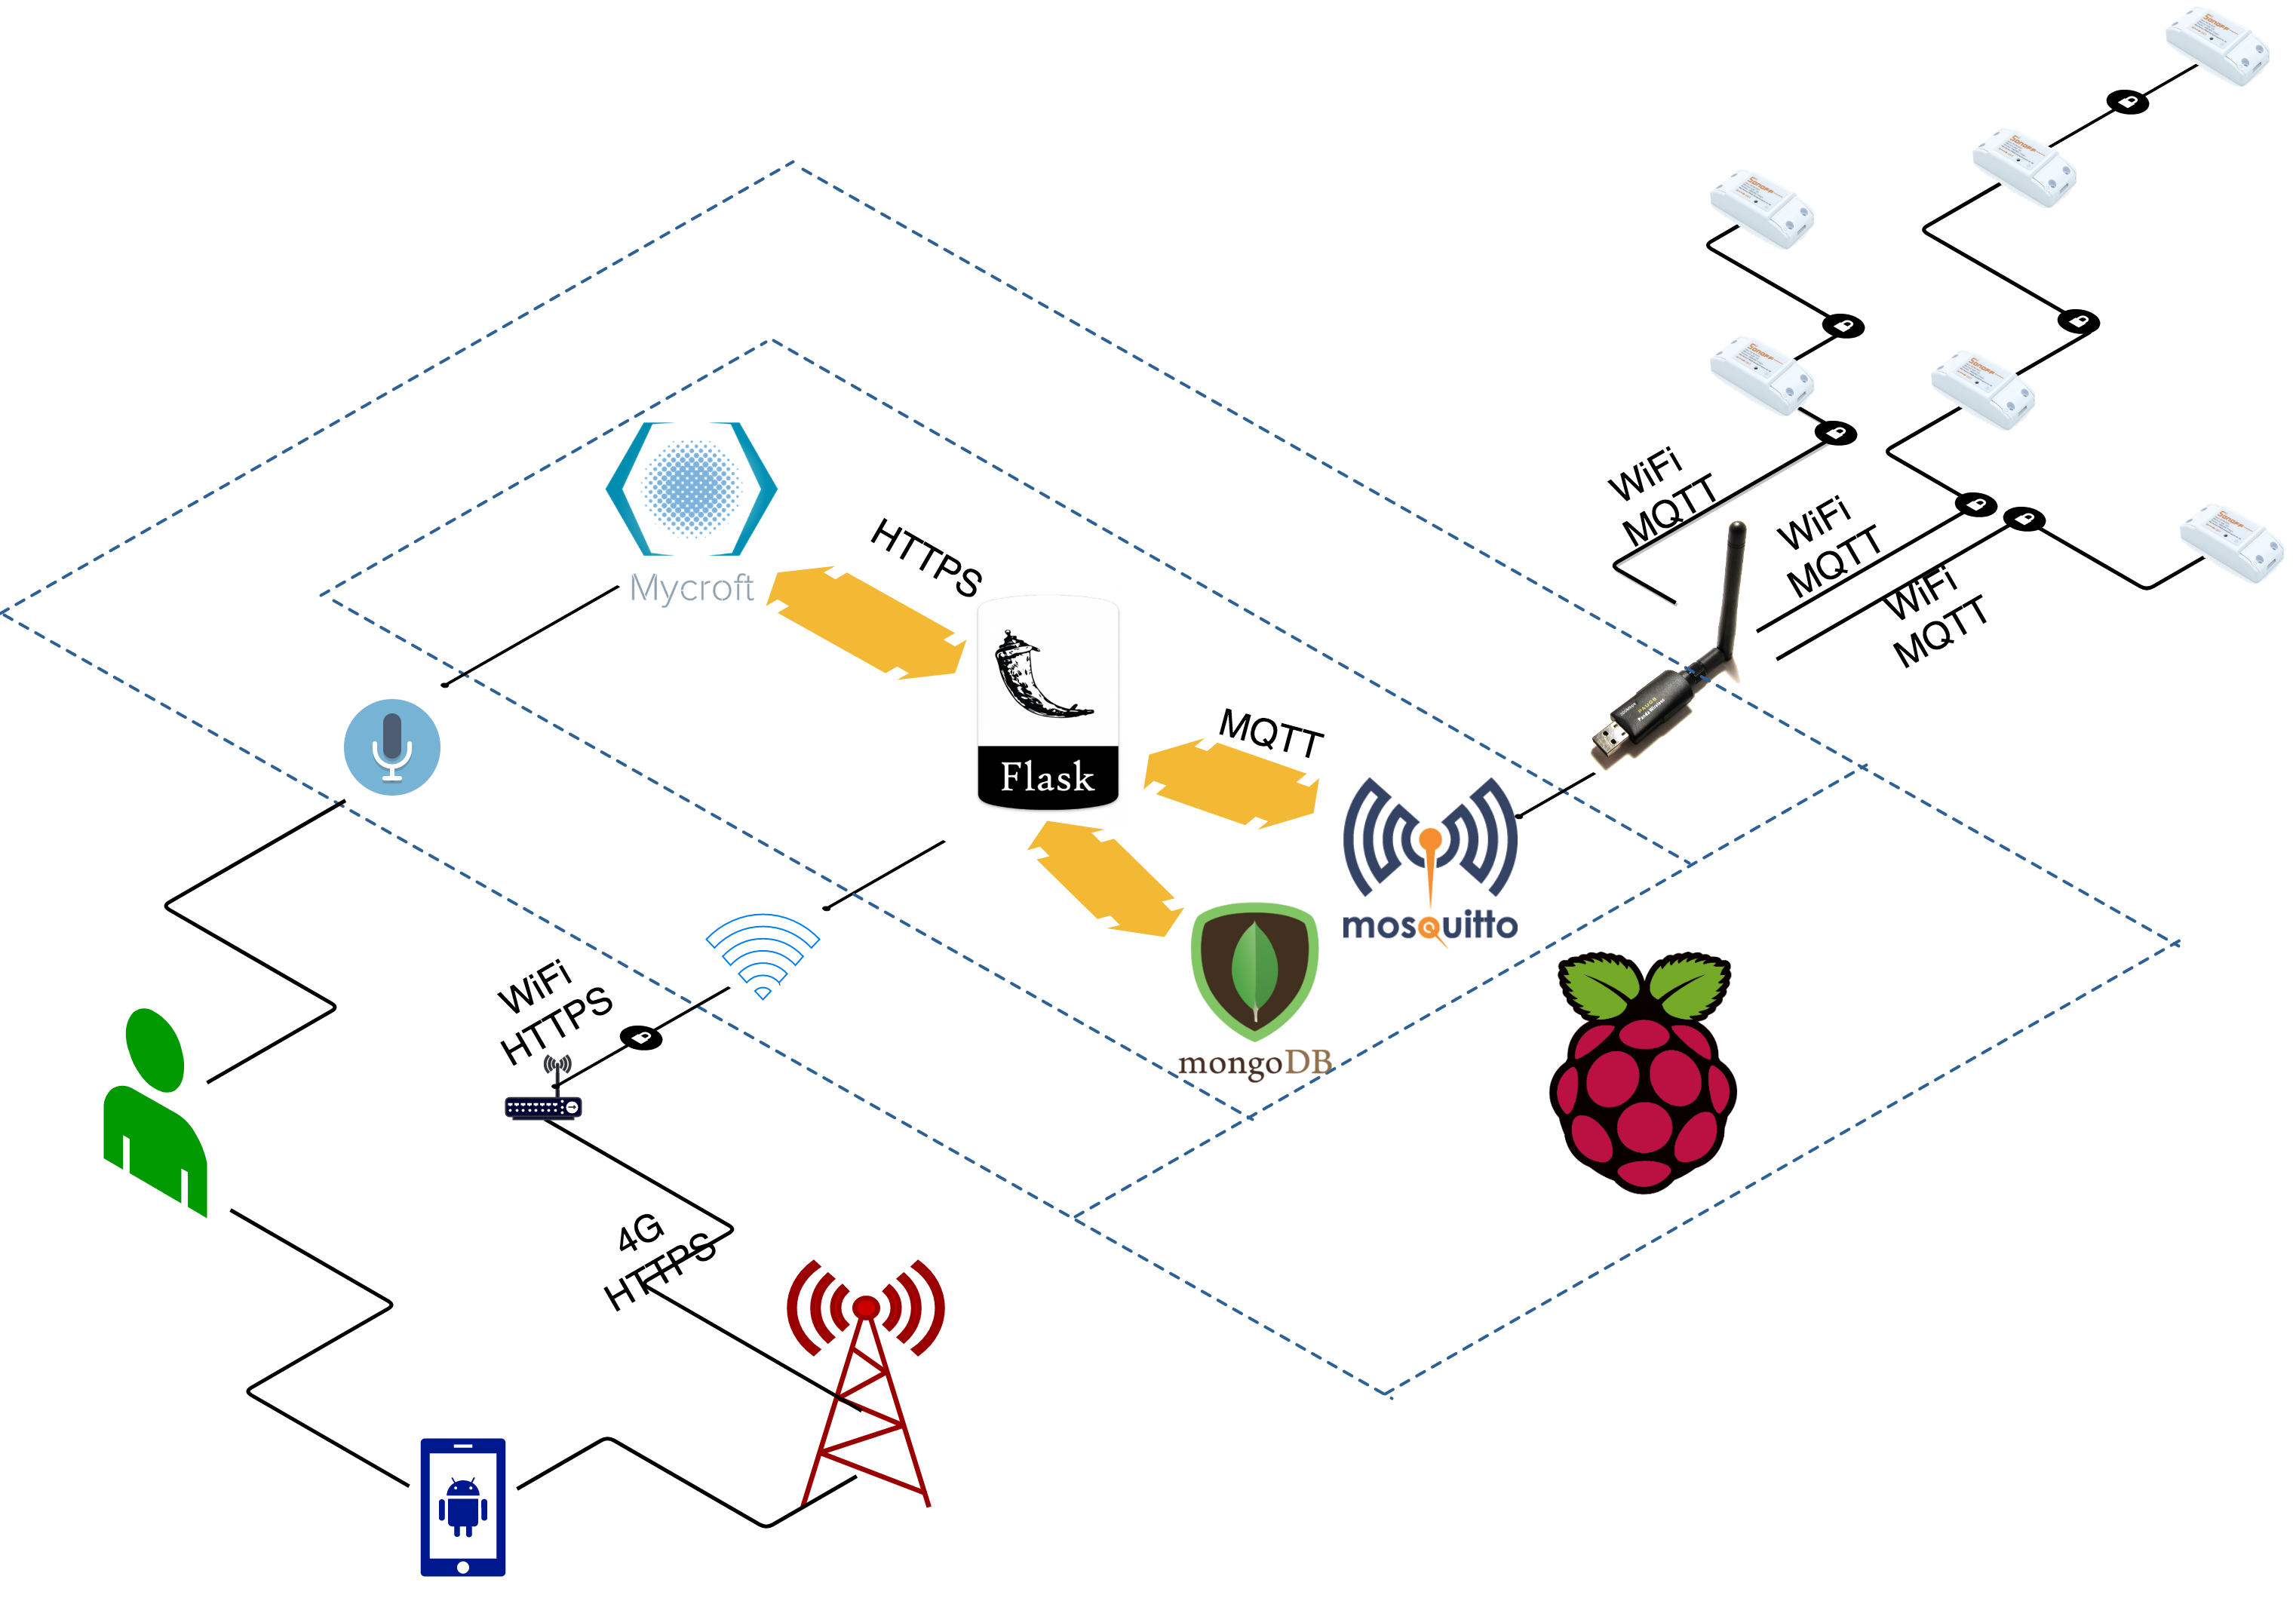
\includegraphics[width=0.8\textwidth, keepaspectratio]{images/arquitectura-intro}
  \caption{\textit{Arquitectura general del sistema construido.}}
  \label{fig:dude-arq}
\end{figure}

El usuario interactúa con el servidor Flask a través de alguna de las interfaces brindadas. Luego el servidor se encarga de interactuar con los interruptores inteligentes según corresponda.

\section{Git}
Para el desarrollo de código grupal, es necesario utilizar un controlador de versiones del mismo, ya que es posible que varios desarrolladores quieran efectuar cambios en el mismo archivo, perdiéndose o dañándose parte del código.
Esta herramienta fue diseñada por Linus Torvalds, conocido por iniciar y mantener el desarrollo del kernel de Linux, y en la actualidad es ampliamente utilizada en proyectos con gran extensión de código y varios desarrolladores.
Algunos conceptos básicos a manejar del mismo son:

\begin{itemize}

\item Branch: es una versión paralela a un repositorio, contenida en el mismo pero permite realizar cambios sin modificar la versión "oficial", una vez terminados y testeados los cambios se pueden aplicar a la versión utilizada por los demás desarrolladores.

\item Clone: es una copia del repositorio que se encuentra alojada en el computador del desarrollador en vez de en el servidor donde se guarda el repositorio.

\item Commit: es un cambio individual de un archivo o varios de ellos, es el equivalente a guardar un cambio, pero en vez de ser en el sistema local de almacenamiento es en git. Esto permite llevar un registro de los cambios y quién los hizo, esta tarea es usualmente facilitada con un mensaje adherido a cada commit con una breve descripción de los cambios. Este registro permite volver a estados anteriores y deshacer cambios incorrectos.

\item Push: Este comando envía los cambios registrados en los commits anteriores, reflejando los mismos en el repositorio remoto para que sean visibles para los demás usuarios.

\item Pull request: son cambios propuestos a un repositorio, realizados por un usuario y aceptados o rechazados por los colaboradores del repositorio en cuestión. Cada pull request cuenta con su propio foro de discusión y es posible requerir cambios antes de aceptar o rechazar el mismo.

\end{itemize}

Para este proyecto se utilizó una estrategia de 2 branches principales y un branch por nueva funcionalidad, las cuales se mencionan a continuación:

\begin{itemize}

\item master: Esta branch aloja checkpoints del proyecto, por lo que el código en la misma debe ser testeado antes de trasladarse y debe tomarse como puntos de referencia en casos de fallo del sistema. Ningún usuario tiene autorización para realizar push a esta branch, por lo que hasta los administradores del proyecto deben abrir un pull request y esperar que este sea aprobado para efectuar cambios.

\item dev: Branch de desarrollo, sale de el último commit de master y de ella se deben abrir las branches de nuevas funcionalidades, es una branch de adaptación de código, por lo que su estado no es tan estable como master. Los usuarios tampoco tienen permitido realizar push directos, por lo que deberán abrir un pull request para mergear las branches de funcionalidades.

\item branches de funcionalidades: son la estrategia a seguir para desarrollar nuevas funcionalidades, los desarrolladores deben ir pusheando sus cambios y al terminar una tarea, recién solicitar reflejar estos cambios en dev.

\end{itemize}

\section{PlatformIO}
Es un IDE creado para un ambiente de desarrollo en IoT. Satisface una necesidad de los programadores a la hora de embarcarse en proyectos de IoT la cual es que hay muchas tecnologías diferentes con las que debe trabajar, esto hace que lograr la configuración correcta para cada una de ellas pueda ser un dolor de cabeza si no se maneja con este IDEs o similares. PlatformIO logra  integrar todo dentro del mismo ambiente de programación.~\cite{PlatformIODocs} 

Por ejemplo, para programar en un board Arduino típicamente se debe descargar  el IDE de Arduino en donde se compila y sube el código. Si para cada board hubiera que hacer lo mismo, y además saber que configuración crearle a cada uno para que funcione con las diferentes librerías que se desea integrar al proyecto, lo cual representa un gran contratiempo. Lo que brinda PlatformIO es la posibilidad de descargar diferentes boards (más de 200) de desarrollo (como Arduino), así como integrar diferentes librerías para cada plataforma y todo de forma intuitiva y fácil desde una interfaz gráfica.

Otro factor positivo es que se integra fácilmente con Atom~\cite{Atom}, que es un IDE conocido y previamente usado por los integrantes del grupo.

La librería mesh que elegimos tiene como dependencias otras librerías y usa una plataforma llamada espressif~\cite{espressif-platformio}. Para configurar esto alcanza descargar el board en PlatformIO, agregar una línea en el archivo de configuración diciendo cual se usa y desde la interfaz gráfica descargar las librerías que son dependencia. 

PlatformIO incluso se encarga de mantener actualizadas las plataformas y librerías en su última versión. Hacer esto manualmente es una pérdida de tiempo.

\begin{figure}[h!]
  \centering
  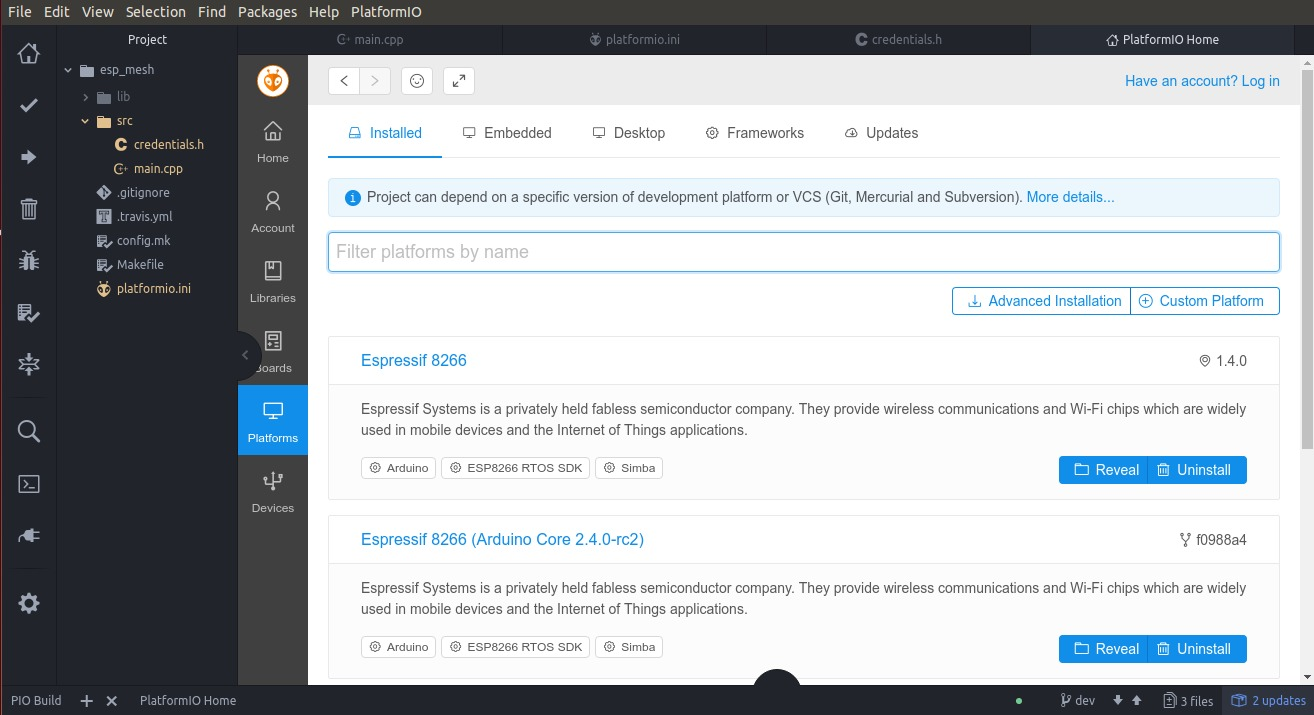
\includegraphics[width=0.8\textwidth, keepaspectratio]{images/platformio}
  \caption{\textit{Interfaz de Atom con PlatfromIO.}}
  \label{fig:atom-plat}
\end{figure}

\section{Protocolos IoT}

\subsection{HTTP}

Hypertext Transfer Protocol o HTTP es un protocolo de capa de aplicación que posibilita el intercambio de comunicación entre cliente y servidor. La última versión fue liberada en el 2015,  descripta en la RFC 7540. Funciona por arriba de la capas TCP/IP y es muy popular. Se basa en operaciones de solicitud/respuesta. Una vez que un cliente se conecta al servidor empieza el intercambio de solicitudes y respuestas entre ambos.

\subsection{CoAP}

CoAP (Constrained Application Protocol) está definido en la RFC 7228 y fue creado con la concepción de ser un protocolo ligero apto para la transferencia de datos en nodos con un procesamiento limitado y redes también limitadas, como todo protocolo de IoT. Así como HTTP, este protocolo está basado en una arquitectura REST (Representational State Transfer), pero tiene una diferencia fundamental frente a HTTP la cual es que HTTP utiliza como capa de transporte TCP y CoAP UDP. 

Para ilustrar lo anteriormente dicho:

\begin{figure}[h!]
  \centering
  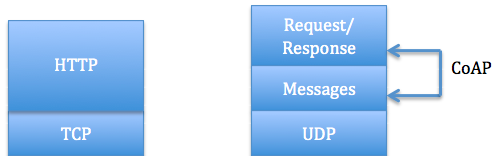
\includegraphics[width=0.8\textwidth, keepaspectratio]{images/http-coap}
  \caption{\textit{Capaz de stack de protocolos CoAP~\cite{HTTP_CoAP_img}.}}
  \label{fig:http_coap}
\end{figure}

\subsection{MQTT}

Message Queue Telemetry Transport (MQTT) es un estándar ISO (ISO/IEC PRF 20922) que funciona sobre TCP/IP y está pensado para correr en dispositivos con bajo nivel de procesamiento como los ESP8266. 

\begin{figure}[h!]
  \centering
  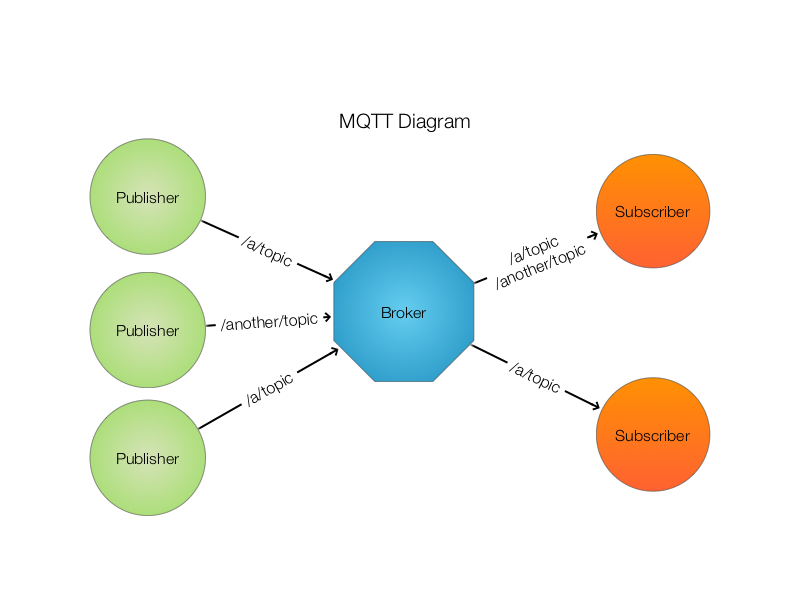
\includegraphics[width=0.6\textwidth, keepaspectratio]{images/mqtt-diagram}
  \caption{\textit{Diagrama de red MQTT.~\cite{MQTT_img}.}}
  \label{fig:mqtt-diag}
\end{figure}

Como se ve en la figura~\qref{fig:mqtt-diag} la arquitectura de este protocolo consiste de 3 partes fundamentales: el publisher, el broker y el subscriber. El broker es el encargado de recibir los mensajes procesar a qué topic está dirigido ese mensaje que envía el publisher y mandarlos hacia los subscribers que estén escuchando los mensajes de ese topic particular. Un topic es un String como puede ser \lstinline[columns=fixed]{"this/is/a/topic"} y subscribers que escuchan los mensajes de ese topic son los que están suscritos a ese topic. Así como CoAP, este protocolo es M2M por lo que sirve para conectar los clientes que son los nodos al servidor.

Hay conceptos introductorios que son necesarios aclarar a la hora de entender el funcionamiento del protocolo. Estos son:

\subsubsection{Cliente:}

En MQTT un cliente es cualquier dispositivo que esté conectado a la red MQTT. 

\subsubsection{Patrón Publish/Subscribe:}

En este patrón, el dispositivo que publica (publisher) un mensaje desconoce qué dispositivo/s escuchan este mensaje. El cliente publica a un broker que es el encargado de mandar ese mensaje a los subscribers, que son los  dispositivos están interesados en escuchar ese mensaje. Esto quiere decir que los publishers no saben de la existencia de los subscribers y viceversa. Por lo general los clientes pueden publicar mensajes y suscribirse a topics. 

\subsubsection{Topics:}
Un topic es un string en formato UTF-8, el cual es usado por el broker para filtrar los mensajes para cada cliente, el mismo consiste de varios niveles que se usan para poder publicar y suscribirse a varios topics, de forma general o específica, de manera fácil e intuitiva. Cada nivel está separado por un separador (\lstinline[columns=fixed]{/}). 

\begin{figure}[h!]
  \centering
  
\includegraphics[width=0.8\textwidth, keepaspectratio]{images/topic-basics}
  \caption{\textit{Composición de un topic MQTT.~\cite{MQTTEssentials5}.}}
  \label{fig:topic-basics}
\end{figure}

Esta solución es extremadamente liviana y no requiere previa inicialización por parte del broker, por lo que el mismo aceptará suscripciones y publicaciones a cualquier topic válido.
Algunos detalles a tener en cuenta:

\begin{itemize}

\item Los niveles no pueden ser un string vacío:
\lstinline[columns=fixed]{"mqtt//topic/"}
\item Los mismos son case-sensitive:
\lstinline[columns=fixed]{"mqtt/topic != mqtt/Topic"}
 
\item Un separador marca un nuevo nivel:
\lstinline[columns=fixed]{"mqtt/topic != mqtt/topic/"}

\end{itemize}

\subsubsection{Wildcards:}

En algunos casos es útil suscribirse a topics con determinadas características, pero que no se sabe con exactitud el topic completo, para esto existen las llamadas wildcards, que representan uno o varios niveles de nombre desconocido.

\begin{itemize}

\item De un nivel: \lstinline[columns=fixed]{"+"}

\begin{figure}[h!]
  \centering
  
\includegraphics[width=0.8\textwidth, keepaspectratio]{images/topic-wildcard-plus}
  \caption{\textit{Uso de la wildcard "+".~\cite{MQTTEssentials5}.}}
  \label{fig:topic-wildcard-plus}
\end{figure}

Cualquier topic que respete la estructura con un string en lugar de la wildcard será reconocido como un match, por ejemplo si se suscribe a \lstinline[columns=fixed]{"myhome/groundfloor/+/temperature"} se recibirán o no los mensajes publicados a los siguientes topics:

\begin{figure}[h!]
  \centering
  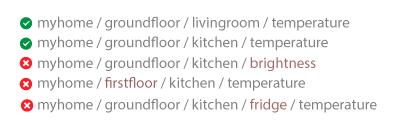
\includegraphics[width=0.8\textwidth, keepaspectratio]{images/topic-wildcard-plus-example}
  \caption{\textit{Topics ejemplo.~\cite{MQTTEssentials5}.}}
  \label{fig:topic-wildcard-plus-example}
\end{figure}

\item Multinivel: \lstinline[columns=fixed]{"#"}

A diferencia la wildcard de un nivel, esta wildcard sólo puede ser colocada al final de un topic y suscribe a todo topic que comience igual que el topic suscrito, sin importar que tantos niveles tenga a continuación.

\begin{figure}[h!]
  \centering

  \begin{subfigure}[b]{0.45\textwidth}
    
\includegraphics[width=0.8\textwidth, keepaspectratio]{images/topic-wildcard-hash}
	  \caption{\textit{Uso de la wildcard "\#".~\cite{MQTTEssentials5}.}}
	  \label{fig:topic-wildcard-hash}
  \end{subfigure}
  ~
  \begin{subfigure}[b]{0.45\textwidth}
    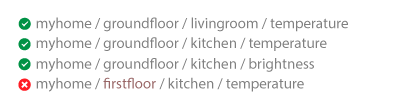
\includegraphics[width=0.8\textwidth, keepaspectratio]{images/topic-wildcard-hash-example}
	  \caption{\textit{Topics ejemplo.~\cite{MQTTEssentials5}.}}
	  \label{fig:topic-wildcard-hash-example}
  \end{subfigure}

  
\end{figure}

\item Topics que comienzan con \lstinline[columns=fixed]{"$"}

Aparte de los caracteres mencionados, el otro que tiene un funcionamiento especial es el \lstinline[columns=fixed]{"$"}, la función que cumple es que, cuando un topic comienza con este carácter, entonces no será posible suscribirse al mismo utilizando los wildcards anteriores, esto es asá ya que estos topics son reservados para estadísticas internas de MQTT, y los clientes no tienen permitido publicar en dichos topics.

\end{itemize}

\section{Sonoff}

\subsection{SPIFFS} \label{sec-SPIFFS}

A pesar de que en el chip ESP8266~\cite{esp8266} el sistema de ficheros(o filesistem, FS) este guardado en el mismo chip que el firmware, cambiar el programa por un nuevo script no modificará el FS. Esto es gracias a la sectorización del espacio virtual del chip como se muestra en el diagrama~\qref{lst:SPIFFS}.

\begin{figure}[thp]
\centering
\begin{tabular}{c}
\begin{lstlisting}[language=bash]
|--------------|-------|---------------|--|--|--|--|--|
^              ^       ^               ^     ^
Sketch    OTA update   File system   EEPROM  WiFi config (SDK)
\end{lstlisting}
\end{tabular}
\caption{\textit{Diagrama de SPIFFS en memoria}}
\label{lst:SPIFFS}
\end{figure}

En el caso del chip que viene integrado en los dispositivos Sonoff que se utilizaron en este proyecto, el tamaño total del chip es de 1Mb y los tamaños que se pueden asignar al FS son 64kb, 128kb, 256kb, 512kb.

Algunas de las funciones básicas para el manejo de SPIFFS son:

\textbf{begin}
\begin{lstlisting}[language=bash]
SPIFFS.begin()
\end{lstlisting}
Este método monta el sistema de archivos SPIFFS, debe ser invocado antes de intentas utilizar ninguna API del FS. Retorna \lstinline[columns=fixed]{true} o \lstinline[columns=fixed]{false} según si el montaje fue correcto o no.

\textbf{format}
\begin{lstlisting}[language=C]
SPIFFS.format()
\end{lstlisting}
Este método formatea el FS, puede ser llamado antes o después de \textbf{begin}.

\textbf{open}
\begin{lstlisting}[language=C]
SPIFFS.open(path, mode)
\end{lstlisting}
Abre un archivo. \lstinline[columns=fixed]{path} debe ser la ruta absoluta empezando con una barra (eg. \lstinline[columns=fixed]{/dir/filename.txt}). \lstinline[columns=fixed]{mode} es un string que especifica el modo de acceso, los valores posibles son \lstinline[columns=fixed]{"r", "w", "a", "r+", "w+", "a+"}. Significando estos lo mismo que para \lstinline[columns=fixed]{fopen} en C.

Devuelve un archivo, para chequear que un archivo se haya abierto correctamente, se debe usar un operador booleano.
\begin{lstlisting}[language=C]
File f = SPIFFS.open("/f.txt", "w");
if (!f) {
    Serial.println("file open failed");
}
\end{lstlisting}

\textbf{exists}
\begin{lstlisting}[language=C]
SPIFFS.exists(path)
\end{lstlisting}
Devuelve \lstinline[columns=fixed]{true} si \lstinline[columns=fixed]{path} existe, \lstinline[columns=fixed]{false} en caso contrario.

\textbf{remove}
\begin{lstlisting}[language=C]
SPIFFS.remove(path)
\end{lstlisting}
Remueve un archivo dado su \lstinline[columns=fixed]{path}. Retorna \lstinline[columns=fixed]{true} o \lstinline[columns=fixed]{false} según si el archivo fue correctamente removido o no.


\section{USB TTL Serial}

\subsection{USB TTL Serial Adapter}
Para borrar el código inicial con el que vienen instalados los Sonoff era necesaria una conexión desde el USB de la computadora o dispositivo donde se encuentra el código hacia la UART del ESP8266.

\begin{figure}[h!]
  \centering
  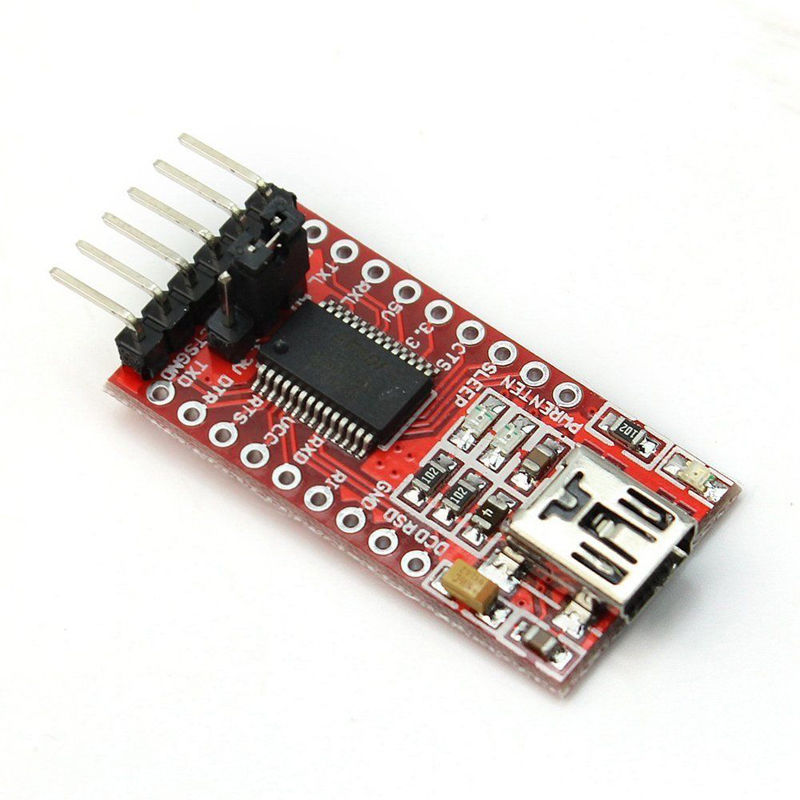
\includegraphics[width=0.6\textwidth, keepaspectratio]{images/usb-serial-adapter}
  \caption{\textit{USB Serial Adapter.~\cite{USBSerialAdapter}.}}
  \label{fig:usb-serial-adapter}
\end{figure}

Para lograrlo, se compraron dispositivos llamados adaptadores USB a TTL serial. De un lado se le conecta un cable mini USB y del otro lado se conectan jumpers que salen de los pines VCC, GRD, Tx, Rx, mientras que se dejan otros 2 pines libres que son el DTR y el CTS. Este chip tiene un jumper para elegir si la salida es de 3,3V o 5V.


\subsection{USB TTL Serial Cable}

Otra posibilidad que se consideró fueron cables USB a TTL serial que como se ve en la figura (x) no tienen ningún elemento activo.

\begin{figure}[h!]
  \centering
  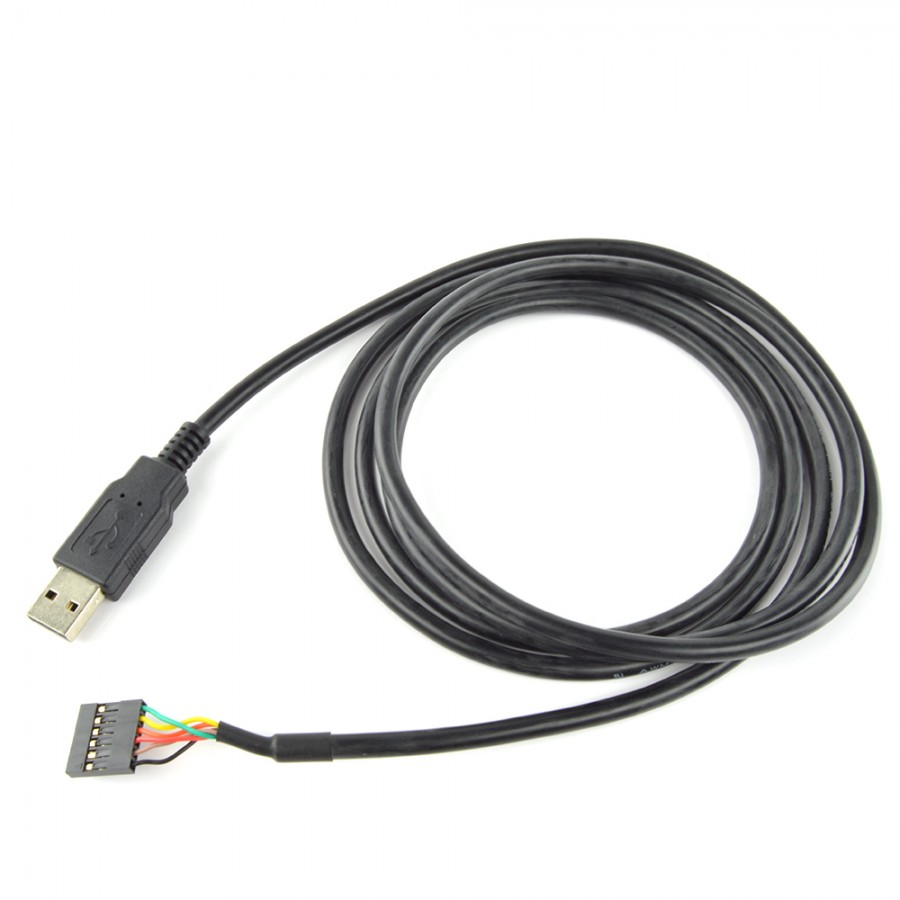
\includegraphics[width=0.5\textwidth, keepaspectratio]{images/usb-serial-cable}
  \caption{\textit{USB Serial Cable.~\cite{USBSerialCable}.}}
  \label{fig:usb-serial-cable}
\end{figure}

\section{Mini Procesadores}

\subsection{Rapsberry Pi 3}

Los Raspberry Pi  (RPi) son computadoras que vienen en un solo circuito (single-board computer), incluyen el microprocesador, la memoria, los input/outputs, la conexión HDMI. Fueron creados en el Reino Unido educar acerca de computación así como para integrar sistemas donde se necesite hardware de bajo costo. Raspberry Pi ha ganado popularidad por todas las prestaciones que da, para el poco costo que tiene.

\begin{figure}[h!]
  \centering
  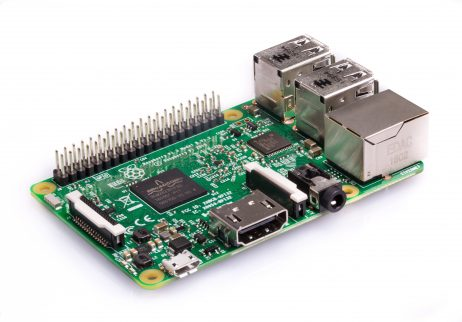
\includegraphics[width=0.5\textwidth, keepaspectratio]{images/rpi3}
  \caption{\textit{Raspberry Pi 3.~\cite{RPi3}.}}
  \label{fig:rpi3}
\end{figure}

Se han desarrollado varios modelos, el que se utiliza en el proyecto es el Raspberry Pi 3 Model B es más reciente.
Requiere una tarjeta microSD, su procesador es de 1,2GHz, memoria RAM de 1Gb y cuenta con las siguientes características entrada Ethernet (RJ-45), 17 GPIOs, alimentación de 5V a través de micro USB o GPIO, salida HDMI, 1 GB de RAM, CPU 64-bit quad-core ARMv8, 4 puertos USB.
Este modelo trae integrado WiFi 802.11n y Bluetooth 4.1.
Su precio es de aproximadamente USD 40.

\subsection{Raspberry Pi 2 B}

La tarjeta de memoria que se le coloca cambia de SD a microSD y el procesador es de 900MHz. Este modelo no cuenta con módulo de WiFi ni Bluetooth integrado, por lo que se debe conectar un dongle en caso de requerir estas características. A pesar de esto, su precio es igual o mayor que el RPi 3.

\begin{figure}[h!]
  \centering
  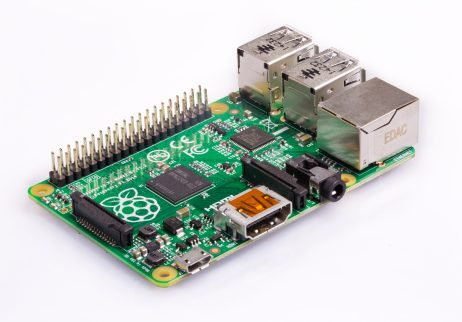
\includegraphics[width=0.5\textwidth, keepaspectratio]{images/rpi2}
  \caption{\textit{Raspberry Pi 2.~\cite{RPi2}.}}
  \label{fig:rpi2}
\end{figure}

\subsection{Banana Pi 3}
Este single-board computer fue influenciado fuertemente por el RPi en su diseño, este modelo es más potente que el RPi 3, con un procesador de 1,8 GHz y memoria RAM de 2Gb, además de contar con memoria flash integrada de 8Gb, lo cual se ve reflejado en su precio que asciende a USD 80. 

\begin{figure}[h!]
  \centering
  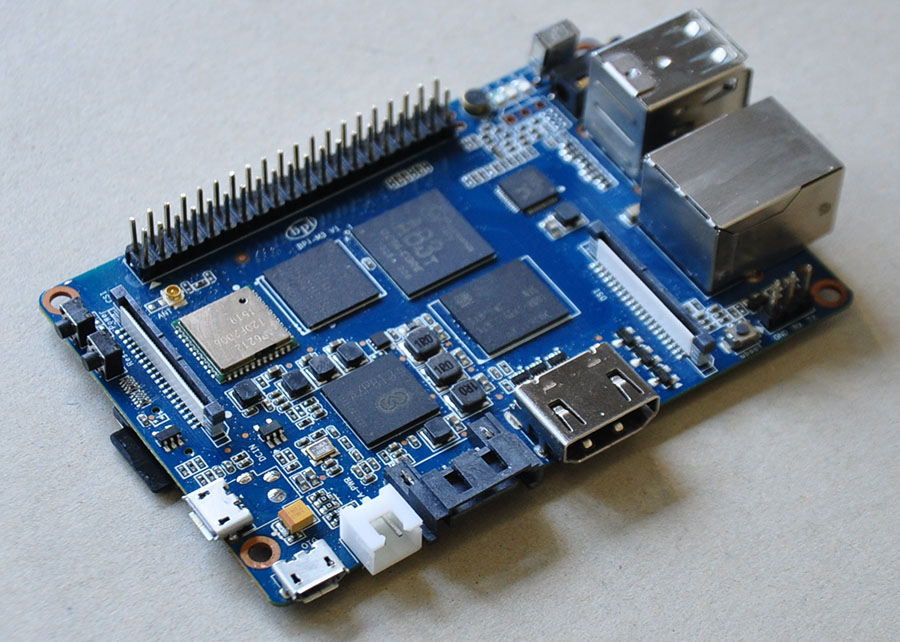
\includegraphics[width=0.5\textwidth, keepaspectratio]{images/bpi3}
  \caption{\textit{Banana Pi M3.~\cite{Banana3}.}}
  \label{fig:bpi3}
\end{figure}

\subsection{BeagleBone Black}
Esta plataforma cuenta con similares características que las anteriores, procesador de 1Ghz, memoria de 512MB, incluyendo también una aceleradora gráfica de 3D y un acelerador NEON de punto flotante, haciéndolo altamente performante para cálculos vectoriales. Sus conexiones son USB, Ethernet, HDMI , 2x 46 pin headers. Su valor es de aproximadamente USD 63.

\begin{figure}[h!]
  \centering
  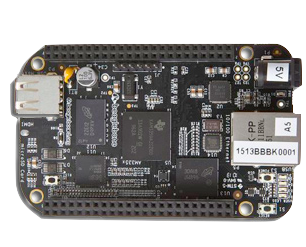
\includegraphics[width=0.4\textwidth, keepaspectratio]{images/bbb}
  \caption{\textit{BeagleBone Black.~\cite{BeagleB}.}}
  \label{fig:bbb}
\end{figure}

\section{Python}
\subsection{pip}
Es un sistema de gestión de paquetes utilizado para instalar y administrar paquetes escritos en Python. Presenta una manera fácil y rápida de instalar paquetes, siendo su interfaz amigable e intuitiva. Algunos comandos son:

\begin{itemize}
\item Instalar un paquete:
\begin{lstlisting}[language=bash]
  $ pip install <nombre del paquete>
\end{lstlisting}	

\item Desinstalar un paquete:
\begin{lstlisting}[language=bash]
  $ pip uninstall <nombre del paquete>
\end{lstlisting}
	

\item Mostrar paquetes instalados:
\begin{lstlisting}[language=bash]
  $ pip list
\end{lstlisting}
	

\item Instalar paquetes indicados en un archivo de requerimientos:
\begin{lstlisting}[language=bash]
  $ pip install -r requirements.txt
\end{lstlisting}

\end{itemize}

\subsection{virtualenvs}

Esta es una herramienta ampliamente utilizada por desarrolladores Python, la misma permite aislar el ambiente de desarrollo del resto de los paquetes Python instalados en el computador del desarrollador. Esto facilita el control de versión de paquetes y permite que el ambiente de desarrollo y producción sean tan similares como sea posible. 
La creación y uso de un virtual env (venv) es muy sencilla, a continuación se muestran los comandos a utilizar:

\begin{itemize}
\item Instalar la herramienta virtualenvwrapper:
\begin{lstlisting}[language=bash]
  	$ pip install virtualenvwrapper
	$ export WORKON_HOME=~/Envs
	$ mkdir -p $WORKON_HOME
	$ source /usr/local/bin/virtualenvwrapper.sh
\end{lstlisting}	

\item Crear un ambiente virtual:
\begin{lstlisting}[language=bash]
  $ mkvirtualenv env1
\end{lstlisting}
	
\item Para instalar un paquete en el venv se debe primero activar el mismo:
\begin{lstlisting}[language=bash]
  $ workon env1
\end{lstlisting}
	
\item Y luego instalar el paquete normalmente:
\begin{lstlisting}[language=bash]
  $ pip install <nombre del paquete>
\end{lstlisting}

\item Para salir de un venv:
\begin{lstlisting}[language=bash]
  $ deactivate
\end{lstlisting}

\end{itemize}

\section{Flask}
Se puede leer la descripción "Flask is a micro web development framework for Python."~\cite{FlaskDocs} en la página oficial de Flask, pero qué significa esto?

"Micro" no significa que toda la aplicación web deba estar contenida en un sólo archivo de Python (aunque bien podría estarlo), ni significa que Flask carece de funcionalidades. El término "micro" se refiere a que Flask tiene como objetivo mantener el núcleo simple pero extensible, lo que es sumamente útil en casos como el de este proyecto, donde se tiene componentes de hardware con capacidades limitadas, y Flask permite agregar sólo las funcionalidades necesarias, ahorrando recursos que otras soluciones menos flexibles y customizables con funcionalidades fijas consumirían.
Una frase que describe muy bien a esta implementación es que "Flask puede ser todo lo que necesitas y nada más." 
Para lograr esto, Flask soporta extensiones para agregar todas las funcionalidades que se necesites como si fueran implementadas por él mismo. Algunas de las librerías disponibles permiten integración con bases de datos, validación de formularios, manejo de subida de archivos, varias tecnologías open source de autenticación, entre otras.

Otra de las características de Flask que lo hacen atractivo para proyectos de desarrollo es la facilidad con la que se agregan o intercambian estos componentes, ya que se pueden tomar decisiones en el proceso de desarrollo pudiendo reutilizar gran parte del código, por ejemplo un cambio de que base de datos utilizar afectaría al servidor únicamente en modificar la extensión a utilizar.

\section{MongoDB}
Hay muchas bases de datos de las que elegir. La razón de esta cantidad de opciones es que difieren en sus objetivos: algunas son buenas realizando consultas complejas, otras tienen un tiempo de consultas muy bajo, algunas pueden escalar fácilmente y llegar a contener petabytes de información.
Estas son una parte importante en cualquier aplicación y la gran decisión a tomar es la de utilizar una clásica base de datos relacional o el nuevo tipo, usualmente llamadas "NoSQL".
MongoDB es una base de datos NoSQL cuya etimología proviene de la palabra "humongous" que significa enorme, que permite desarrollar soluciones ágiles y escalables, características que se adhieren perfectamente con el cometido de este proyecto.
A diferencia de las bases de datos relacionales, guarda los datos en documentos en formato JSON con un esquema dinámico. 
Esto significa que no se debe definir la estructura de estos documentos antes de utilizar la base de datos y que además los mismos pueden ir variando con el tiempo, posibilitando la reutilización de los datos si se decide agregar nuevos tipos de elementos.

Algunos conceptos que se podrían comparar en estas arquitecturas son los siguientes~\cite{MongoDBDocs}:
\begin{table}
    \centering
    \begin{tabular}{ | l | l |}
    \hline
	MySQL & MongoDB \\ \hline
	Table & Collection \\ \hline
	Row & Document \\ \hline
	Column & Field \\ \hline
	Joins & Embedded documents, linking \\ \hline
    \end{tabular}
    \caption{\textit{Comparación de conceptos MongoDB vs BDD relacionales.}.}
    \label{tab:mongo-compare}
\end{table}

\section{React} \label{react-section}
React es una librería de JavaScript desarrollada por Facebook para construir interfaces de usuario. Se basa en la construcción mediante componentes reutilizables, los cuales la librería se encarga de actualizar según cambie el estado al que están relacionados. Estas características hacen de React una opción muy atractiva a la hora de desarrollar aplicaciones web, ya que es fácil de debuggear el código y replicar estados de falla de las aplicaciones.

Otro aspecto de esta librería que la coloca en la cima de las opciones de las empresas, tanto startups como empresas del Fortune 500~\cite{reactjs}, es la capacidad de construir aplicaciones móviles nativas con React Native~\cite{reactnative}, utilizando como lenguaje de desarrollo JavaScript~\cite{js}, uno de los lenguajes más populares actualmente, además de las librerías React y React Native.
La ventaja de esta forma de desarrollar aplicaciones móviles es que a diferencia de PhoneGap y otros wrappers de aplicaciones web, con react native no se construye una aplicación híbrida, sino que se desarrolla con las mismas piezas que utilizando Objective-C o Java, sólo que estos bloques se consolidan usando JavaScript y React.
Esto permite acceder a más funcionalidades específicas de los dispositivos móviles y hace que la aplicación sea apreciablemente más veloz y performante.

\section{Cron}
Cron es un administrador de procesos que es utilizado en Unix. Se encarga de que estos procesos se corran a intervalos constantes de tiempo o a horas específicas ambos determinados por las personas que tengan permisos para crear o editar estos crones. Solo los usuarios que están en el archivo cron.allow son los que pueden crear crones en sus respectivos crontabs. 

El archivo crontab contiene los comandos que se ejecutan, así como la hora o frecuencia con que se corren, como se puede ver a continuación:
Donde la estructura es la siguiente:

\begin{lstlisting}[language=bash]
.--------------- minuto (0-59) 
|  .------------ hora (0-23)
|  |  .--------- dia del mes (1-31)
|  |  |  .------ mes (1-12) 
|  |  |  |  .--- dia de la semana (0-6) (domingo=0 o 7) 
|  |  |  |  |
*  *  *  *  *  comando a ejecutar
\end{lstlisting}

\section{Apache HTTP Server}

Es un servidor web HTTP de código abierto que tiene más de 20 años de creación. Es extremadamente popular, siendo el servidor HTTP más usado y es altamente configurable.  Es multiplataforma, que abarca entre otras, a Unix. Al ser de código abierto y esté hace tanto tiempo en funcionamiento lo hace una opción confiable del punto de vista de la seguridad y que sea fácil conseguir ayuda al tener un problema. https://en.wikipedia.org/wiki/Apache_HTTP_Server.

Los carpetas básicas donde se guarda la información de configuración son: sites-available, sites-enabled. Archivos básicos de configuración son: apache2.conf (nombre en Ubuntu), ports.conf.

En el archivo ports.conf se puede encontrar los puertos en los que escucha el servidor apache. Por defecto solo está habilitado el puerto 80. 

El archivo apache2.conf puede contener toda la configuración del sistema. Por un tema de modularidad y orden se acostumbra a diseminar la configuración en otros archivos.

La carpeta sites-available contiene archivos que definen los hosts virtuales del servidor. El  contenido de estos archivos son lo que direccionan el pedido del usuario cuando accede al servidor. Esto depende de cómo hace el llamado (URL, puerto, ruta) . 

La carpeta sites-enabled contiene los archivos disponibles de sites-available. Son los únicos que tiene en cuenta Apache.

Finalmente, hay una carpeta que no es de configuración pero es de gran importancia. Esta es /var/www/html/ que es donde se ubica todo el código del servidor.

fuente 
https://www.digitalocean.com/community/tutorials/how-to-configure-the-apache-web-server-on-an-ubuntu-or-debian-vps

\section{Amazon EC2}

Amazon Elastic Compute Cloud (Amazon EC2) es un servicio brindado por Amazon Web Services. Brindan un entorno virtualizado para trabajar en la nube. Se puede elegir de un conjunto de imágenes de máquinas virtualizadas con las cuales empezar  a trabajar. A su vez, se brinda la posibilidad de elegir las características de esa computadora como memoria, almacenamiento y capacidad de red de las instancias. A esto se le llama tipo de instancia. También, cuenta con un firewall virtual que se le aplica a una o varias de esas máquina virtuales. Se brinda una IP estática para ese equipo junto con un dominio. 

Al firewall virtual se lo llama Amazon EC2 Security Groups y al crear uno se le puede aplicar a varias instancias (computadoras virtuales). Se le puede añadir un conjunto de reglas para que sean respetadas en varias instancias. Por defecto, solo viene habilitado el SSH para que el usuario se pueda conectar al equipo.

Este servicio tiene un computadoras gratuitas por el primer año, con poco procesamiento, ram y red limitada. De esta forma, si se necesita un servidor con pocos requerimientos de procesamiento y red, se puede usar este de para virtualizar el contenido del mismo y no tener que preocuparse por la alimentación del servidor o por los elementos físicos del mismo como si se tuviera físicamente dentro del hogar o un datacenter.

https://docs.aws.amazon.com/es_es/AWSEC2/latest/UserGuide/concepts.html


\section{Mycroft}
Mycroft es el primer asistente virtual open source, y está diseñado para ser ejecutado en una computadora personal y hasta en un Raspberry Pi. este software open source está a total disposición para ser modificado, extendido o mejorado. 
La instalación del mismo incluye algunos skills básicos, algunas órdenes que se pueden hacer incluyen:

\begin{itemize}

\item ``Hey Mycroft, what time is it?''

\item ``Hey Mycroft, what time is it in Paris?''

\item ``Hey Mycroft, what time is it in Melbourne?''

\item ``Hey Mycroft, what's the weather?''

\item ``Hey Mycroft, set an alarm for 30 minutes.''

\item ``Hey Mycroft, what's my IP address?''

\item ``Hey Mycroft, tell me a joke.''

\item ``Hey Mycroft, tell me about chocolate.''

\item ``Hey Mycroft, tell me about Linux.''

\end{itemize}

Se pueden agregar nuevos skills del repositorio generado con las contribuciones de la comunidad.~\cite{MycrofSkills}
